\documentclass[sigconf,review=false,anonymous=false]{acmart}
\settopmatter{printacmref=false}
\setcopyright{none}
\acmConference[CS 544 Project]{CS 544 Machine Learning in Production}{Fall 2026}{University of Illinois Chicago}
\acmYear{2026}\acmDOI{}\acmISBN{}
\renewcommand\footnotetextcopyrightpermission[1]{}
\pagestyle{plain}
\usepackage{booktabs}
\usepackage{multirow}
\usepackage{xspace}
\usepackage{graphicx}
\graphicspath{{../report/figures/}}

\newcommand{\sys}{\textsc{RagRepair}\xspace}
\newcommand{\INS}{\texttt{INSUFF\-ICIENT}\xspace}

\setlength{\emergencystretch}{1.5em}
\begin{document}

\title{What Reaches the Model? Trace-Based Diagnosis and Repair of Component Faults in RAG Pipelines}

\author{Sina Gogani Khiabani}
\affiliation{\institution{University of Illinois Chicago}\city{Chicago}\state{IL}\country{USA}}
\email{sgoga3@uic.edu}
\author{Verya Monjezi}
\affiliation{\institution{University of Illinois Chicago}\city{Chicago}\state{IL}\country{USA}}
\author{Ali Hoseinpour}
\affiliation{\institution{University of Illinois Chicago}\city{Chicago}\state{IL}\country{USA}}

\begin{abstract}
Retrieval-augmented generation (RAG) services fail not only in retrieval and generation but in
the code between them: templates truncate passages, serving runtimes silently cut prompts that
exceed their context window, indexes keep outdated document versions, and query encoders drift
from the encoder the index was built with. We inject six such faults into a complete RAG service
running on a laptop and compare twelve runtime repair policies, under a budget of two extra model
calls, on 150 HotpotQA questions with Llama-3.2-3B. Generic repairs fail: retry barely changes
success under faults (26.8\% to 27.6\%), and a self-check with the model's own verifier lowers it to
20.7\% while breaking 24.3\% of correct answers. Applying every repair on every request reaches
46.4\% but breaks 15.9\% of correct answers and makes a serving fault worse than doing nothing.
Trace checks, computed from data the service already logs (rendered versus retrieved text, tokens
sent versus tokens processed, duplicate document versions, retrieval confidence), recover 55.9\%
with 1.9\% damage, and a diagnose policy built on them reaches 56.9\% (+30.1 points over no repair,
95\% CI [24.8, 35.7]). Whether an answer is judged unsupported by the model itself, by a MiniCheck
grounding classifier, or by text match matters far less than whether the repair fixes the context.
In simulated request streams, trace checks detect a faulty deploy a median of 4 requests after it
ships; model-based signals need tens of requests or never alarm. A regression suite built from
observed failures replays in seconds from recorded responses and fails whenever a diagnostic is
disabled.
\end{abstract}

\keywords{retrieval-augmented generation, fault injection, runtime monitoring, repair, ML in production}

\maketitle

\section{Introduction}

A retrieval-augmented generation (RAG) service is a pipeline: a retriever finds passages, glue code
assembles them into a prompt, a serving runtime runs the model, and an index holds the documents.
Evaluation frameworks for RAG score the retrieved context and the final
answer~\cite{es2024ragas,saadfalcon2024ares,ru2024ragchecker}. In production, however, evidence can
be lost \emph{between} those two points. A government help-desk assistant lost its system prompt and
its top-ranked documents for weeks because the serving runtime silently kept only the tail of a
prompt that exceeded its default context window~\cite{musetoiu2026ragal}; users of a popular RAG
platform report the same problem when the model server ignores the configured
window~\cite{ragflow_ollama_ctx}. Template code that truncates passages, an index that still holds
an outdated version of an updated document~\cite{ouyang2025hoh}, and a query encoder that no longer
matches the encoder the index was built with are similar failures: the retriever may work, the model
may work, and the answer is still wrong.

When answers look wrong, a common runtime response is generic: retry, or ask the model whether its
answer is supported and regenerate if not. Such repairs spend calls on the generator even when the
generator is not the component that failed, and LLMs are known to be unreliable at verifying their
own outputs without external feedback~\cite{huang2024selfcorrect}. This paper asks a practical
question for teams operating RAG services: \emph{when a pipeline component fails, which runtime
repair helps, what does it break, and what does it cost?}

We study this with a fault-injection harness around a small but complete RAG service running
locally. We inject six faults motivated by reported incidents at four pipeline stages (retrieval,
prompt assembly, serving, index content), and compare twelve repair policies under a fixed budget
of two extra model calls. The policies range from generic (retry, self-check) to
\emph{trace-based}: checks computed from what the service already logs, such as whether the rendered
prompt is shorter than the retrieved text or whether the server processed fewer tokens than were
sent. We measure success under faults, damage to answers that were correct, abstention when the
evidence is gone, and cost. We address four questions:
\begin{description}
\item[RQ1] How do generic, blanket and trace-based repairs compare under component faults?
\item[RQ2] Does the verifier or the repair action matter more? We cross \{LLM self-verifier,
MiniCheck grounding classifier~\cite{tang2024minicheck}, text match\} with \{regenerate on the
same passages, repair the context\}.
\item[RQ3] How quickly do trace checks and model-based signals detect a faulty deploy in a
request stream?
\item[RQ4] Can a regression suite built from observed failures catch regressions in the repair
logic itself?
\end{description}

On 150 held-out HotpotQA questions with Llama-3.2-3B, trace-based diagnosis raises success under
faults from 26.8\% to 56.9\% (+30.1 points, 95\% CI [24.8, 35.7]) while breaking 4.7\% of correct
clean answers; trace checks alone account for almost all of the gain. A generic LLM self-check
lowers success to 20.7\% and breaks 24.3\% of correct clean answers. Applying every repair on every
request reaches 46.4\%, breaks 15.9\% of correct clean answers, and makes the serving fault worse
than doing nothing (6.0\% vs.\ 30.0\%). Trace checks detect each global fault a median of 4
requests after a deploy; the model's own verifier needs tens of requests and often never alarms.
A 35-case regression suite, replayed from recorded responses in seconds, fails whenever one of
the diagnostics is disabled.

\paragraph{Contributions.} (1) A fault-injection study of RAG runtime repair that treats prompt
assembly and serving as components that can fail; (2) a budget-matched comparison of twelve
repair policies that accounts for damage and abstention; (3) evidence that cheap, model-free trace
checks recover most of the benefit and detect faulty deploys fastest, while model self-verification
is harmful at this scale; and (4) an open, laptop-scale artifact with record/replay regression tests
for LLM pipelines.

\section{Related Work}\label{sec:related}

\paragraph{RAG failures and evaluation.} Barnett et al.\ catalog seven failure points of RAG systems
and argue that RAG can only be fully validated in operation~\cite{barnett2024seven}. RAGAS, ARES and
RAGChecker score retrieval and generation quality~\cite{es2024ragas,saadfalcon2024ares,ru2024ragchecker};
RAGChecker separates retriever and generator errors with claim-level metrics. Chen et al.\ study 654
configuration issues in ten RAG systems and find that root causes often sit in a different stage
than the symptoms~\cite{chen2026configuring}. Kim et al.\ apply metamorphic testing to RAG under
corpus changes~\cite{kim2026knowledge}. These works measure the retrieved context and the answer;
we additionally treat prompt assembly and serving, the glue code that Sculley et al.\ identify as a
source of hidden debt~\cite{sculley2015debt}, as components that can fail, and we test at runtime
rather than offline.

\paragraph{Repair and self-correction.} Self-RAG trains a model to critique its retrievals and
generations~\cite{asai2024selfrag}; CRAG uses a retrieval evaluator to trigger corrective
retrieval~\cite{yan2024crag}; Doctor-RAG localizes failures in agentic RAG trajectories and repairs
from the earliest failure point~\cite{jiao2026doctorrag}. Huang et al.\ show that LLMs cannot
reliably self-correct reasoning without external feedback~\cite{huang2024selfcorrect}. We compare
lightweight, training-free policies under a fixed call budget and measure what they break.

\paragraph{Grounding, staleness and abstention.} MiniCheck provides small, accurate grounding
classifiers~\cite{tang2024minicheck}. HoH shows that outdated information coexisting with current
information degrades RAG~\cite{ouyang2025hoh}. RefusalBench evaluates when grounded models should
refuse~\cite{muhamed2026refusalbench}.

\paragraph{ML in production.} The ML Test Score lists monitoring and testing practices for
production ML~\cite{breck2017mltestscore}; Ma et al.\ argue for slice-based regression tests of
evolving LLM APIs~\cite{ma2024prompt}; Dutta et al.\ show that aggregate accuracy hides changed
predictions after model compression~\cite{dutta2024accuracy}, the motivation for our clean-damage
measure. Our monitoring and record/replay tests follow the practices described by
K\"astner~\cite{kastner2025mlip}.

\section{Study Design}\label{sec:design}

\subsection{System under test}
The service answers a question in three steps. (1) \emph{Retrieval}: dense retrieval with
\texttt{bge-small-en-v1.5}~\cite{xiao2023cpack} over a fixed passage store, top $k{=}5$. A BM25 index
over the same store is available as a lexical fallback. (2) \emph{Prompt assembly}: each passage is
rendered as \texttt{[P$i$] title (last updated date)} followed by its text, and the instruction asks
for the shortest possible answer plus the ids of supporting passages, or \INS{}.
(3) \emph{Serving}: a 4-bit instruction-tuned model served locally with MLX~\cite{mlx2023}, greedy
decoding. The service logs a trace for every call: retrieved documents with their similarity scores
and metadata, the passages exactly as rendered, the number of prompt tokens it sent and the number
the server reports as processed, and the raw output. Repair policies see this trace and nothing else;
they never see the fault label or the gold answer.

\subsection{Data}
We use the HotpotQA distractor validation set~\cite{yang2018hotpotqa}. We keep \emph{bridge}
questions whose answer string occurs in exactly one of the question's ten paragraphs, in a gold
supporting sentence, and drop answers with annotation artifacts. The first 1{,}200 such questions
(seeded shuffle) define the store: all their paragraphs, deduplicated by title (11{,}737 passages).
Of these, 664 have both gold paragraphs in the clean dense top-5; this filter guarantees that in the
clean condition the evidence is present, so each injected fault is the only reason it goes missing.
We draw 30 development and 150 test questions and exclude every question used in an earlier
prototype of this study. Each passage carries a ``last updated'' date (2023--2024). For the stale
fault, each question's answer passage also has an \emph{old version}, dated three to six years
earlier, in which the answer value is replaced by a plausible wrong value: numbers and dates are
shifted by rule; entity answers are rewritten by a local 7B model (e.g., Sam Waterston $\to$ Tom
Hanks) and checked to differ from the gold answer.

\subsection{Faults}
Table~\ref{tab:faults} lists the six faults. Each models a failure reported for deployed RAG
services, and none targets the answer passage directly except \emph{absent}, where abstaining is the
correct behavior.

\begin{table}[t]
\caption{Injected faults, by pipeline stage.}\label{tab:faults}
\small
\begin{tabular}{@{}p{1.55cm}p{3.15cm}p{2.9cm}@{}}
\toprule
Fault & Injection & Production cause \\
\midrule
encoder & queries embedded with \texttt{all-MiniLM-L6-v2}~\cite{reimers2019sbert}; index built with \texttt{bge-small} & query service falls back to a library default encoder \\
truncation & template cuts every passage to its first 100 characters & \texttt{text[:max\_chars]} misconfiguration \\
overflow & server keeps only the last 512 prompt tokens & unset context window, e.g.\ \texttt{num\_ctx} default~\cite{musetoiu2026ragal,ragflow_ollama_ctx} \\
stale & old version of the answer passage indexed beside the current one; retrieval ranks both & index not deduplicated after an update~\cite{ouyang2025hoh} \\
absent & answer passage removed from the index & content gap \\
enc.+trunc. & encoder and truncation together & independent faults co-occur \\
\bottomrule
\end{tabular}
\end{table}

\subsection{Signals and repair policies}
\emph{Trace checks} are computed from the trace with no model call: (i) \emph{truncation}, a rendered
passage is shorter than the retrieved text; (ii) \emph{version conflict}, two passages share a title;
(iii) \emph{overflow}, the server processed fewer prompt tokens than were sent; (iv) \emph{low
retrieval}, the top dense similarity is below the 5th percentile of clean traffic, calibrated on
467 held-out questions. Each check has a matching repair: render in full, keep the newest version,
fit the passages to the window the server reported, or fall back to BM25. \emph{Support checks}
decide whether an answer is grounded: a text-match check (the answer appears in the passages), the
model's own verifier (``Is the proposed answer correct and directly supported by the passages?
SUPPORTED/UNSUPPORTED''), or MiniCheck-RoBERTa-Large~\cite{tang2024minicheck}, a 355M-parameter
grounding classifier run on the passages packed into 400-token chunks. MiniCheck's model and claim
format were chosen on prototype development data; its thresholds were set on the development split by
rules fixed in advance (0.5, MiniCheck's default, to trigger a repair; the 2nd percentile of scores
of correct grounded answers, 0.01, to abstain). The support check of the proposed policy (text
match) was also chosen on the development split; the other two remain as comparison arms.

Table~\ref{tab:policies} lists the policies. All start from the same initial answer and may make at
most two more model calls; LLM verifier calls count against this budget, MiniCheck calls do not
(their time is reported separately). \emph{Diagnose} applies the repairs indicated by the trace
checks, then checks support; while the answer is unsupported and budget remains it widens
retrieval to 10, then adds BM25 results, regenerating after each step; if the final answer is
still clearly unsupported it returns \INS{}. The self-check and diagnose variants
form a factorial design: \{LLM verifier, MiniCheck\} $\times$ \{regenerate on the same passages,
repair the context\}, plus text match with context repair.

\begin{table}[t]
\caption{Repair policies (budget: two extra model calls).}\label{tab:policies}
\small
\begin{tabular}{@{}p{2.25cm}p{5.4cm}@{}}
\toprule
Policy & Behavior \\
\midrule
No repair & deployed pipeline \\
Retry & if \INS{}, resample at temperature 0.7 \\
Self-check (2 verifiers) & verify the answer (LLM or MiniCheck); if unsupported, regenerate on the same passages with a hint \\
Repair-all & always: dense top-10 $\cup$ BM25 top-5, full rendering, newest versions, regenerate \\
Trace checks only & trace checks and their repairs; no support check \\
Diagnose (3 support checks) & trace checks, then a support check (text match, LLM, or MiniCheck) with re-check after each repair, retrieval ladder, abstention \\
\quad ablations & proposed (text match) variant without re-check, without abstention, without trace checks \\
\bottomrule
\end{tabular}
\end{table}

\subsection{Measures and statistics}
\emph{Success} is a correct answer in the answerable conditions and \INS{} in
\emph{absent}. Correctness is exact match after normalization (number words mapped to digits),
token F1 $\geq 0.8$, or the gold phrase inside a short prediction; other predictions go to a local
answer-equivalence judge (Qwen2.5-7B) that sees only the question, gold answer and prediction. On
the prototype, 197 of 203 audited judge decisions agreed with a manual audit; we report results with
string matching alone as a sensitivity check. \emph{Success under faults} averages the five
answerable fault conditions per question. \emph{Clean damage} is the share of clean questions
answered correctly at first and wrongly after the policy~\cite{dutta2024accuracy}. Costs are model
calls, prompt tokens and GPU seconds per case. All comparisons are paired by question: 95\% intervals
are percentile bootstraps over questions (2{,}000 resamples), per-condition tests are exact McNemar.

\subsection{Model and setup}
The generator is Llama-3.2-3B-Instruct~\cite{grattafiori2024llama3}, 4-bit, served with MLX on one
MacBook Pro (M4, 16\,GB); this paper reports one model, and extending the study to
Qwen2.5-7B~\cite{qwen2025qwen25} and Gemma-2-9B~\cite{gemma2024gemma2} is ongoing
(Section~\ref{sec:threats}). A response cache keyed by model, prompt and sampling settings lets
policies that issue the same prompt share generations and makes every run replayable.

\section{Results}\label{sec:results}

\begin{table}[t]
\caption{Test results (Llama-3.2-3B, 150 questions). Faults: success under the five answerable
faults (\%). Dmg.: correct clean answers broken (\%). Abst.: abstention when the answer passage is
absent (\%). Tok.: prompt tokens per case.}\label{tab:main}
\small
\begin{tabular}{lrrrr}
\toprule
 & \multicolumn{4}{c}{Llama-3.2-3B} \\
\cmidrule(lr){2-5}
Policy & Faults & Dmg. & Abst. & Tok. \\
\midrule
No repair & 26.8 & 0.0 & 38.7 & 0.7k \\
Retry & 27.6 & 0.0 & 34.0 & 0.9k \\
Self-check (LLM) & 20.7 & 24.3 & 60.7 & 1.5k \\
Self-check (MiniCheck) & 22.4 & 12.1 & 55.3 & 1.0k \\
Repair-all & 46.4 & 15.9 & 20.0 & 2.4k \\
Trace checks only & 55.9 & 1.9 & 38.0 & 1.2k \\
\textbf{Diagnose (text match)} & 56.9 & 4.7 & 28.0 & 1.5k \\
Diagnose (LLM verifier) & 57.2 & 11.2 & 28.0 & 2.3k \\
Diagnose (MiniCheck) & 59.3 & 7.5 & 29.3 & 2.1k \\
\midrule
\quad $-$ re-check & 53.1 & 5.6 & 30.0 & 1.3k \\
\quad $-$ abstention & 59.9 & 1.9 & 23.3 & 1.5k \\
\quad $-$ trace checks & 31.9 & 3.7 & 30.0 & 1.3k \\
\bottomrule
\end{tabular}

\end{table}

\begin{figure*}[t]
\centering
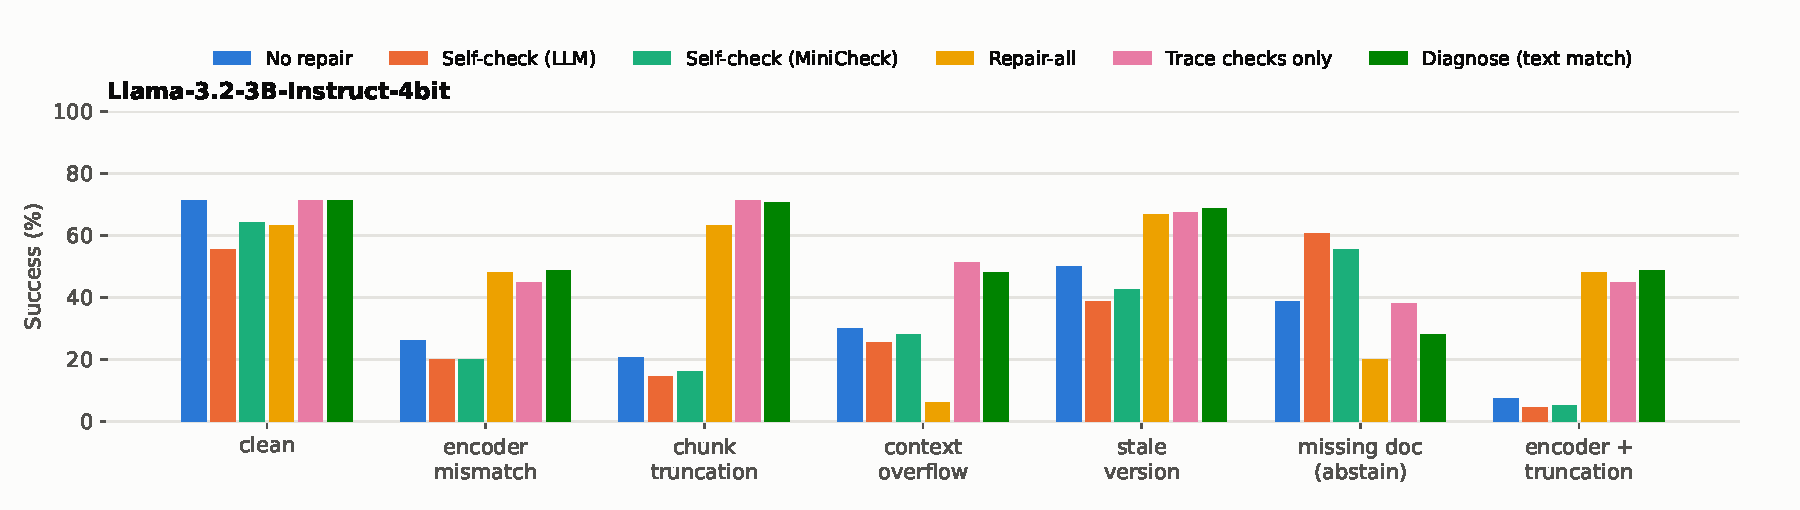
\includegraphics[width=\textwidth]{success_by_condition.pdf}
\caption{Success by condition for six policies (Llama-3.2-3B, 150 test questions). In
\emph{absent}, success means abstaining.}\label{fig:conditions}
\end{figure*}

\subsection{RQ1: Which repairs help?}
Table~\ref{tab:main} and Figure~\ref{fig:conditions} summarize the comparison; all differences
below are paired by question.

\paragraph{Generic repairs do not help.} With no repair the service answers 71.3\% of clean
questions but only 26.8\% [22.7, 31.2] under faults. Retry changes little (27.6\%): it only fires
on \INS{} and resamples the same broken prompt. Self-check is worse than no repair
(20.7\%) and breaks 24.3\% of correct clean answers, almost always by turning them into
\INS{} after its verifier calls them unsupported.

\paragraph{Blanket repair helps but breaks things.} Repair-all (wider dense retrieval plus BM25,
full rendering, newest versions, on every request) reaches 46.4\% under faults. It costs a second
call with 3.6$\times$ the prompt tokens of the deployed pipeline, breaks 15.9\% of correct clean
answers, and lowers abstention on unanswerable questions from 38.7\% to 20.0\%. Under the serving
fault it is far worse than doing nothing (6.0\% vs.\ 30.0\%): its longer prompt loses even more to
the server's silent cut, so the repair amplifies the fault.

\paragraph{Trace checks do most of the work.} The four trace checks with their matching repairs
reach 55.9\% [49.7, 62.0] under faults while breaking 1.9\% of correct clean answers, at 1.72 calls
and 1.2k prompt tokens per case. Diagnose adds a support check, a retrieval ladder and abstention:
56.9\% [50.7, 63.1], +30.1 points over no repair [24.8, 35.7] and +10.5 over Repair-all [6.4, 14.9],
but only +1.1 [$-$2.0, 4.0] over trace checks alone. The ablations explain why. Removing the trace
checks drops success to 31.9\% ($-$25.1 [$-$30.0, $-$20.3]): a support check that sees only the answer
cannot tell a template bug from a retrieval miss, and widening retrieval does not undo truncation or
overflow. Re-checking support after a repair is worth +3.9 points [1.9, 6.0], mostly under the
encoder fault, where the first fallback is often not enough. Abstention costs 2.9 points under
faults [1.1, 5.3] and raises clean damage from 1.9\% to 4.7\%, while recovering only 4.7 points of
appropriate abstention.

\paragraph{The checks are precise.} The truncation and overflow checks fired on every faulty case
and on no clean case; the version check fired on 86\% of stale cases (the outdated copy was in the
prompt in 91\%); the low-retrieval check fired on every encoder-fault case and, by construction of
its threshold, on 4\% of clean cases, where its BM25 fallback did no measurable harm.

\paragraph{Repairs reduce abstention.} When the answer passage is missing, the deployed pipeline
abstains 38.7\% of the time; Diagnose abstains 28.0\% ($p{=}0.004$). The retrieval ladder adds
passages, and the model then finds a plausible but wrong entity to name. Only the self-check
policies abstain more (55--61\%), and they pay for it with clean damage.

\begin{figure}[t]
\centering
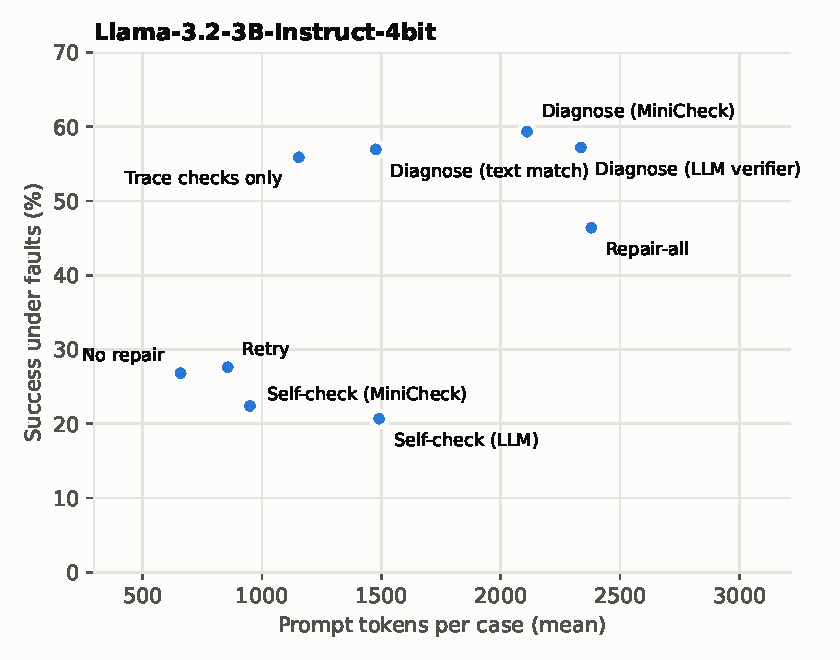
\includegraphics[width=\columnwidth]{cost_vs_success.pdf}
\caption{Success under faults versus prompt tokens per case.}\label{fig:cost}
\end{figure}

\subsection{RQ2: Verifier or repair?}
Table~\ref{tab:factorial} crosses the decision of \emph{whether} an answer is unsupported with
\emph{what happens next}. Regenerating on the same passages fails with either verifier
(20.7\%, 22.4\%); repairing the context succeeds with any of the three (56.9--59.3\%). The repair
action, not the verifier, determines recovery. The verifier mainly determines damage: the LLM
self-verifier breaks the most correct answers in either column.

Table~\ref{tab:support} evaluates the gates directly on 700 non-abstaining initial answers. The LLM
self-verifier keeps only 26.3\% of correct, grounded answers. MiniCheck is better balanced (AUROC
0.67) but still rejects nearly half of the good answers at its default threshold; multi-hop answers
whose support spans two passages are hard for a 355M-parameter grounding classifier.
Is this a small-model artifact? On a stratified sample of 240 of the same answers we asked Claude
Haiku~4.5 the identical verifier question. It keeps 71.7\% of good answers and catches 82.4\% of bad
ones (balanced accuracy 0.77), against 20.7\% and 91.2\% (0.56) for the 3B model's self-verifier and
0.63 for MiniCheck. A stronger verifier would remove most of the false alarms that made self-check
destroy correct answers. It would not make self-check repair anything: under truncation, overflow
or a retrieval fault the evidence is not in the passages, so regenerating on them cannot recover
it, which is what the left column of Table~\ref{tab:factorial} shows for both verifiers. Even the
strong verifier is close to chance on truncated passages (0.53), where the question is whether
missing text would have supported the answer.

\begin{table}[t]
\caption{Verifier $\times$ repair. Cells: success under faults / clean damage (\%).}\label{tab:factorial}
\small
\begin{tabular}{llrr}
\toprule
Model & Verifier & Regenerate & Repair context \\
\midrule
Llama-3.2-3B & LLM self-verifier & 20.7 / 24.3 & 57.2 / 11.2 \\
 & MiniCheck & 22.4 / 12.1 & 59.3 / 7.5 \\
 & Text match & -- & 56.9 / 4.7 \\
\bottomrule
\end{tabular}

\end{table}

\begin{table}[t]
\caption{Support checks as gates on initial answers. Good kept: correct, grounded answers judged
supported. Bad caught: other answers judged unsupported.}\label{tab:support}
\small
\begin{tabular}{lrrr}
\toprule
Check & Good kept & Bad caught & Bal.\ acc. \\
\midrule
\multicolumn{4}{l}{\emph{Llama-3.2-3B: 700 initial answers, 285 correct and grounded}} \\
LLM self-verifier & 26.3 & 86.7 & 0.57 \\
MiniCheck $\geq 0.5$ (AUROC 0.67) & 52.6 & 72.8 & 0.63 \\
\midrule
\multicolumn{4}{l}{\emph{Same 240 answers (40 per condition) for all three}} \\
Llama-3.2-3B self-verifier & 20.7 & 91.2 & 0.56 \\
Claude Haiku 4.5, same prompt & 71.7 & 82.4 & 0.77 \\
MiniCheck $\geq 0.5$ & 45.7 & 81.1 & 0.63 \\
\bottomrule
\end{tabular}

\end{table}

\subsection{RQ3: How fast is a faulty deploy detected?}
We simulate 300 request streams per fault: 400 clean requests, then 200 after a deploy that
introduces the fault (the stale fault affects 20\% of post-deploy requests, the others all of them).
A signal alarms when its rate over the last 50 requests exceeds the clean mean plus three standard
deviations. Table~\ref{tab:monitor} and Figure~\ref{fig:monitor} show that trace checks alarm a
median of 4 requests after each global fault and 24 requests after the partial stale fault, with
0.1\% false alarms. MiniCheck needs 18--35 requests for global faults and rarely detects the stale
one. The LLM verifier flags 75\% of \emph{clean} answers, so its alarm threshold is high; it needs
34--93 requests and misses two thirds of overflow deploys. The model's abstention rate is a
reasonable signal for retrieval and truncation faults (7--10 requests), slow for overflow (56) and
poor for stale documents.

\begin{table}[t]
\caption{Detection delay after a faulty deploy: median requests until the first alarm (share of
300 runs with an alarm). --: detected in fewer than half the runs.}\label{tab:monitor}
\small
\begin{tabular}{lrrrr}
\toprule
Fault & Trace & MiniCheck & LLM ver. & Abstain \\
\midrule
encoder & 4 (100\%) & 23 (100\%) & 63 (67\%) & 10 (100\%) \\
truncation & 4 (100\%) & 19 (100\%) & 39 (92\%) & 10 (100\%) \\
overflow & 4 (100\%) & 35 (100\%) & -- & 56 (89\%) \\
stale & 24 (100\%) & -- & -- & -- \\
enc.+trunc. & 4 (100\%) & 18 (100\%) & 34 (99\%) & 7 (100\%) \\
\bottomrule
\end{tabular}

\end{table}

\begin{figure*}[t]
\centering
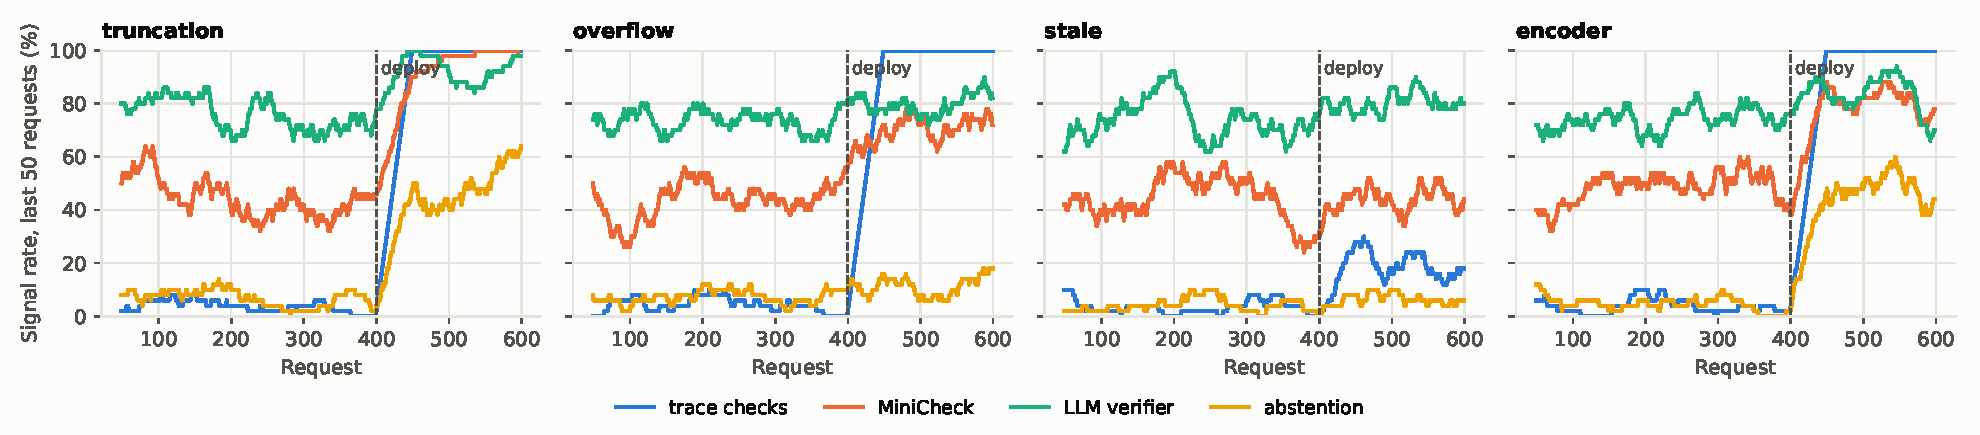
\includegraphics[width=\textwidth]{monitoring_Llama-3.2-3B.pdf}
\caption{Signal rates in one simulated stream per fault; the dashed line marks the deploy.}\label{fig:monitor}
\end{figure*}

\subsection{RQ4: Regression tests from observed failures}
We turned 35 observed cases into a regression suite: five clean questions that must stay correct
and, for each fault, five failures that Diagnose repaired. Because every model response and support
score is cached, the suite replays the full pipeline in about 7 seconds without loading a model;
a code change that alters a prompt or a repair decision misses the cache and fails until it is
re-recorded. To check that the suite has teeth, we disabled one diagnostic at a time and replayed it
on the live model (Table~\ref{tab:mutation}). Every mutation failed exactly the cases of the fault it
covers.

\begin{table}[t]
\caption{Regression suite under mutations of the repair logic (35 cases).}\label{tab:mutation}
\small
\begin{tabular}{lrl}
\toprule
Mutation & Failing & Conditions \\
\midrule
none & 0 & -- \\
no truncation check & 10 & truncation, encoder+truncation \\
no low-retrieval check & 8 & encoder, encoder+truncation \\
no overflow check & 5 & overflow \\
no version check & 4 & stale \\
no re-check after repair & 3 & encoder, encoder+truncation \\
\bottomrule
\end{tabular}
\end{table}

\subsection{Sensitivity to scoring}
The equivalence judge accepted aliases such as ``Bob Iger'' for ``Robert A.\ Iger''. We audited
all 63 of its acceptances on the test set, overturned 13 (it had accepted a related entity, e.g.\
``Greene King'' for ``Bury St Edmunds''), and corrected them; 59 of 60 sampled rejections were
right. With string matching alone, success under faults drops by 8--18 points but every conclusion
holds: Diagnose beats no repair by +24.5 [19.5, 29.9] and Repair-all by +9.9 [5.7, 13.9], trace
checks alone are within +1.3 [$-$0.9, 3.5], and self-check remains the worst policy.

\section{Lessons for Practitioners}\label{sec:lessons}

\paragraph{Log what reaches the model.} The most useful signals were comparisons the service could
make with data it already had: rendered versus retrieved text, tokens sent versus tokens the server
processed, and duplicate document identities in the context. Standard retrieval metrics measure
what was retrieved, not what survived assembly; these checks cost nothing and alarmed within a few
requests of a bad deploy.

\paragraph{Match the repair to the component.} Re-asking the generator on the same broken context
never helped, and doing every repair on every request made the serving fault worse. A repair needs
to know which component failed.

\paragraph{Do not let a small model veto its own answers.} The 3B model's verifier rejected most of
its correct answers. Used as a gate, it destroyed good answers; used as a trigger for context repair,
it cost little recovery but more damage than a text match. A frontier verifier is far better
calibrated, but verification only decides \emph{whether} to act; recovery comes from fixing the
context.

\paragraph{Check again after each repair.} When two faults co-occur, fixing the visible one may not
be enough; re-checking support after a repair recovered several points under the encoder fault.

\paragraph{Treat abstention as a separate requirement.} Repairs that add passages make the model
less willing to say it does not know. None of the policies we tested achieved both high recovery
and high abstention on unanswerable questions.

\section{Threats to Validity}\label{sec:threats}

\paragraph{Construct.} Faults are injected deterministically, and questions were filtered so that
clean dense retrieval finds both supporting passages; real retrieval is noisier and real faults
less tidy. The faults are modeled on reported incidents, but their severity (e.g., a 100-character
truncation, a 512-token window) was chosen by us. The text-match support check works because
HotpotQA answers are extractive spans; abstractive answers would need an entailment model.

\paragraph{Internal.} The proposed policy's support check, MiniCheck's thresholds and the
retrieval-confidence threshold were chosen on development or held-out calibration questions,
disjoint from the test set, by rules fixed before the test run. On the test set the MiniCheck
variant scored slightly higher than the proposed text-match variant (59.3\% vs.\ 56.9\%, difference
not significant), which we report as is. Correctness relies partly on an LLM judge; all of its test
acceptances were audited by the first author's AI assistant and corrected, and a blind audit sheet
for two human annotators is part of the artifact.

\paragraph{External.} We report one 3B model, greedy decoding, one dataset and one retriever.
Larger models verify better: Claude Haiku~4.5 reached 0.77 balanced accuracy as a verifier on our
answers, so self-check with a strong verifier would break fewer correct answers, although it still
cannot recover missing evidence. We measured the strong verifier on a sample only, not as a full
policy. Runs with Qwen2.5-7B and Gemma-2-9B are in progress with the same harness. Costs are measured on one laptop
and are meaningful only relative to each other.

\paragraph{Conclusion validity.} With 150 questions, pooled comparisons have intervals of roughly
$\pm$5 points; several per-condition differences between the stronger policies are not significant.

\section{Conclusion}
We injected six production-motivated faults into a RAG service and compared twelve runtime repair
policies under a fixed call budget. Checks on what actually reached the model, computed from the
service's own trace, recovered most of the lost accuracy, broke few correct answers, and detected
faulty deploys within a handful of requests. Generic self-checking with the model's own verifier
was worse than no repair, and blanket repair amplified a serving fault. The harness, data
construction, recorded responses and regression suite are available for replication.

\paragraph{Artifact.} Code, data construction scripts, recorded model responses, result files and
the regression suite are in the project repository.


\bibliographystyle{ACM-Reference-Format}
\bibliography{refs}

\end{document}
